\documentclass[border=1.5mm]{standalone}
\usepackage[T1]{fontenc}
\usepackage{times}
\usepackage{xcolor}
\usepackage{tikz}
\usetikzlibrary{arrows.meta,calc,positioning,shapes.geometric}

\definecolor{ink}{gray}{0}
\definecolor{line}{gray}{0}
\definecolor{panel}{gray}{0.97}
\definecolor{header}{gray}{0.90}
\definecolor{feedback}{gray}{0}

\newcommand{\entitygroup}[2]{%
  \begin{minipage}{#1}\raggedright
  #2
  \end{minipage}%
}

\begin{document}
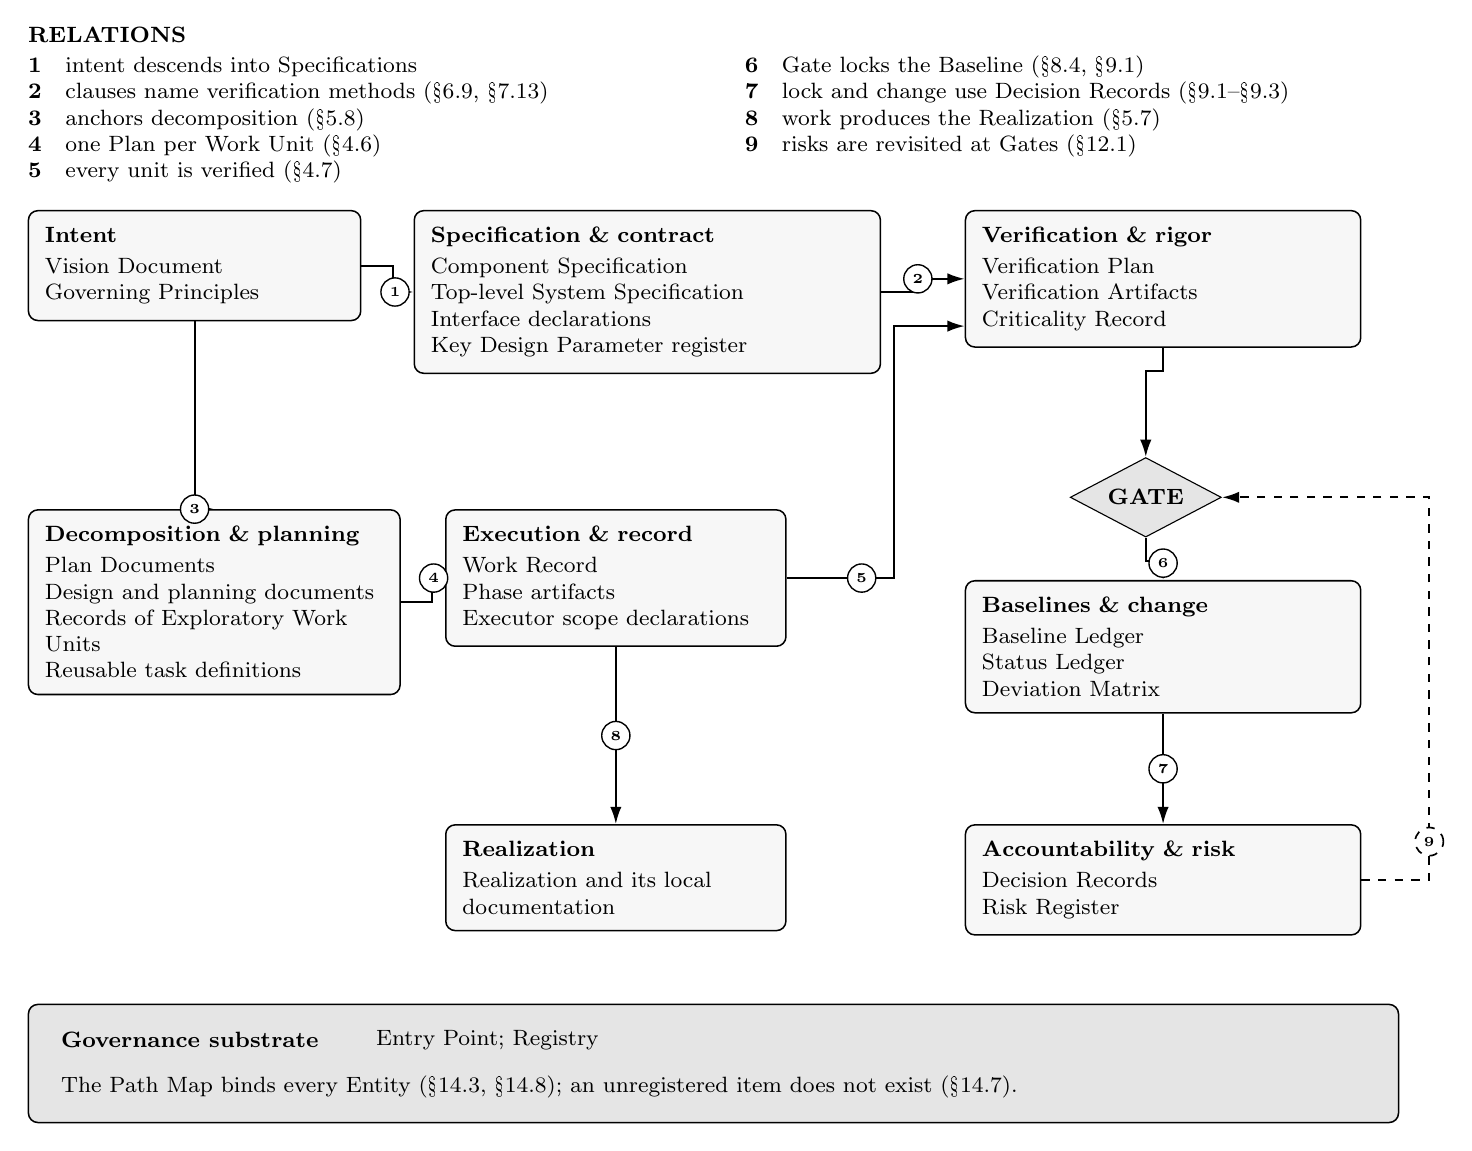
\begin{tikzpicture}[
  x=1mm,
  y=1mm,
  group/.style={
    draw=line,
    rounded corners=1.2mm,
    fill=panel,
    line width=0.55pt,
    inner sep=2.1mm,
    anchor=north west,
    font=\footnotesize,
    text=ink,
    align=left
  },
  relation/.style={-{Latex[length=2.2mm,width=1.45mm]},draw=line,line width=0.75pt},
  feedback relation/.style={-{Latex[length=2.2mm,width=1.45mm]},draw=feedback,line width=0.85pt,dashed},
  marker/.style={circle,draw=line,fill=white,line width=0.5pt,inner sep=0.65mm,font=\tiny\bfseries,text=ink},
  feedback marker/.style={circle,draw=feedback,fill=white,line width=0.6pt,inner sep=0.65mm,font=\tiny\bfseries,text=feedback},
  gate/.style={draw=line,fill=header,diamond,aspect=1.9,inner xsep=1.6mm,inner ysep=0.7mm,font=\footnotesize\bfseries,text=ink}
]

\node[anchor=south west,inner sep=0pt,text=ink] at (3,120) {%
  \begin{minipage}{174mm}\footnotesize
  \textbf{RELATIONS}\\[1.1mm]
  \begin{tabular}{@{}p{83mm}@{\hspace{8mm}}p{83mm}@{}}
  \textbf{1}\quad intent descends into Specifications & \textbf{6}\quad Gate locks the Baseline (\S8.4, \S9.1) \\
  \textbf{2}\quad clauses name verification methods (\S6.9, \S7.13) & \textbf{7}\quad lock and change use Decision Records (\S9.1--\S9.3) \\
  \textbf{3}\quad anchors decomposition (\S5.8) & \textbf{8}\quad work produces the Realization (\S5.7) \\
  \textbf{4}\quad one Plan per Work Unit (\S4.6) & \textbf{9}\quad risks are revisited at Gates (\S12.1) \\
  \textbf{5}\quad every unit is verified (\S4.7) & \\
  \end{tabular}
  \end{minipage}};

\node[group,text width=38mm] (intent) at (3,117) {\entitygroup{38mm}{\textbf{Intent}\\[0.6mm]Vision Document\\Governing Principles}};

\node[group,text width=55mm] (contract) at (52,117) {\entitygroup{55mm}{\textbf{Specification \& contract}\\[0.6mm]Component Specification\\Top-level System Specification\\Interface declarations\\Key Design Parameter register}};

\node[group,text width=46mm] (verify) at (122,117) {\entitygroup{46mm}{\textbf{Verification \& rigor}\\[0.6mm]Verification Plan\\Verification Artifacts\\Criticality Record}};

\node[group,text width=43mm] (planning) at (3,79) {\entitygroup{43mm}{\textbf{Decomposition \& planning}\\[0.6mm]Plan Documents\\Design and planning documents\\Records of Exploratory Work Units\\Reusable task definitions}};

\node[group,text width=39mm] (execution) at (56,79) {\entitygroup{39mm}{\textbf{Execution \& record}\\[0.6mm]Work Record\\Phase artifacts\\Executor scope declarations}};

\node[group,text width=46mm] (baseline) at (122,70) {\entitygroup{46mm}{\textbf{Baselines \& change}\\[0.6mm]Baseline Ledger\\Status Ledger\\Deviation Matrix}};

\node[group,text width=39mm] (realization) at (56,39) {\entitygroup{39mm}{\textbf{Realization}\\[0.6mm]Realization and its local documentation}};

\node[group,text width=46mm] (account) at (122,39) {\entitygroup{46mm}{\textbf{Accountability \& risk}\\[0.6mm]Decision Records\\Risk Register}};

\node[draw=line,rounded corners=1.2mm,fill=header,line width=0.55pt,minimum width=174mm,minimum height=15mm,anchor=south west,text=ink] (governance) at (3,1) {};
\node[anchor=west,font=\footnotesize\bfseries,text=ink] at ($(governance.west)+(3,3.0)$) {Governance substrate};
\node[anchor=west,font=\footnotesize,text=ink] at ($(governance.west)+(43,3.0)$) {Entry Point; Registry};
\node[anchor=west,font=\footnotesize,text=ink] at ($(governance.west)+(3,-3.0)$) {The Path Map binds every Entity (\S14.3, \S14.8); an unregistered item does not exist (\S14.7).};

\draw[relation] (intent.east) -- ++(4,0) |- node[marker,pos=0.55] {1} (contract.west);
\draw[relation] (contract.east) -- ++(4,0) |- node[marker,pos=0.55] {2} (verify.west);

\draw[relation] (intent.south) |- node[marker,pos=0.50] {3} (planning.north);
\draw[relation] (planning.east) -- ++(4,0) |- node[marker,pos=0.55] {4} (execution.west);

\coordinate (verificationtarget) at ($(verify.west)+(0,-6)$);
\coordinate (verificationturn) at ($(verificationtarget)+(-9,0)$);
\draw[relation] (execution.east) -| node[marker,pos=0.35] {5} (verificationturn) -- (verificationtarget);

\node[gate] (gate) at (145,80.5) {GATE};
\draw[relation] (verify.south) -- ++(0,-3) -| (gate.north);
\draw[relation] (gate.south) -- ++(0,-3) -| node[marker,pos=0.55] {6} (baseline.north);

\draw[relation] (baseline.south) -- node[marker] {7} (account.north);
\draw[relation] (execution.south) -- node[marker] {8} (realization.north);

\coordinate (feedbackrail) at (181,80.5);
\draw[feedback relation] (account.east) -| node[feedback marker,pos=0.55] {9} (feedbackrail) -- (gate.east);

\end{tikzpicture}
\end{document}
